\documentclass[../../Thesis.tex]{subfiles}
\usepackage[italian]{babel}

\begin{document}
\chapter{Motivazioni e Lavori Correlati}
In questa sezione della tesi, verranno illustrate in modo approfondito le motivazioni che hanno guidato la scelta del tema di ricerca. Inoltre, saranno presentati e discussi alcuni dei contributi più rilevanti e significativi della letteratura esistente che si sono occupati di tematiche affini.

\section{Motivazioni}
\label{ch:motivations}

Nel 1994, Nick Szabo, un informatico e crittografo, propose la prima descrizione ufficiale degli smart contracts \cite{Szabo_1997}:
 \begin{quotation}
    "Smart contracts combine protocols, users interfaces, and promises expressed via those interfaces, to formalize and secure relationships over public networks. This gives us new ways to formalize the digital relationships which are far more functional than their inanimate paper-based ancestors. Smart contracts reduce mental and computational transaction costs, imposed by either principals, third parties, or their tools."
 \end{quotation}
L'idea di base dietro uno smart contract è che molte clausole contrattuali possono essere incorporate in hardware e software con cui tutti i giorni interagiamo. Un primo esempio di antenato degli smart contracts possono essere considerati i distributori automatici, che erogano un bene (una bevanda) in cambio di un pagamento. Questo processo è automatizzato e non richiede l'intervento di un intermediario. Il distributore automatico rappresenta un contratto con il portatore: chiunque abbia monete può partecipare a uno scambio con il venditore. La cassetta di sicurezza e altri meccanismi di sicurezza proteggono le monete e il contenuto dagli attacchi, sufficientemente da permettere l'installazione redditizia di distributori automatici in una vasta gamma di aree.

\subsection{Blockchain}
Ad oggi, gli Smart Contracts hanno avuto un'ampissima diffusione grazie allo sviluppo  e alla diffusione della tecnologia blockchain. La blockhain è una tecnologia che permette di costruire un ledger distribuito, cioè un registro condiviso e sincronizzato tra tutti i nodi della rete. Questo registro è immutabile e contiene tutte le transazioni che sono state effettuate. La blockchain è stata introdotta per la prima volta nel 2008 da un autore (o un gruppo di autori) sotto lo pseudonimo di Satoshi Nakamoto, come parte del progetto Bitcoin \cite{Bitcoin}. La blockchain, ha queste caratteristiche principali \cite{Blockchain}:
\begin{itemize}
    \item \textbf{Decentralizzazione}: al contrario dei sistemi di transazione centralizzati, in cui ogni transazione deve essere validata da un'autorità centrale, questo non avviene nella blockchain. In una blockchain, le transazioni sono validate da una rete di nodi distribuiti, che lavorano insieme per raggiungere un consenso sulla validità delle transazioni utilizzando un algoritmo di consenso.
    \item \textbf{Persistenza:} le transazioni registrate sulla blockchain sono immutabili e non possono essere modificate una volta che sono state confermate. I blocchi che contengono transazioni invalide vengono immediatamente scoperti e scartati dalla rete. Questo garantisce che il registro sia accurato e affidabile.
    \item \textbf{Anonimità:} ogni utente interagisce con la blockhain con un indirizzo generato, che non rivela la reale indentita dell'utente. Questo garantisce un certo grado di anonimità e privacy. Allo stesso tempo, la blockchain non puo garantire un anonimato totale. 
\end{itemize}
A livello architetturale, la blockhain è una sequenza di blocchi, che tengono una lista completa di record di transazioni, come un ledger pubblicato. Ogni blocco contiene un hash crittografico del blocco precedente, un timestamp e un set di transazioni. Questi blocchi sono concatenati insieme per formare una catena, da cui il nome "blockchain". Il primo blocco di una blockchain è chiamato \emph{blocco genesi} e non ha un blocco precedente. Ogni blocco successivo è collegato al blocco precedente e può avere solo un padre.
\begin{figure}[h!]
    \centering
    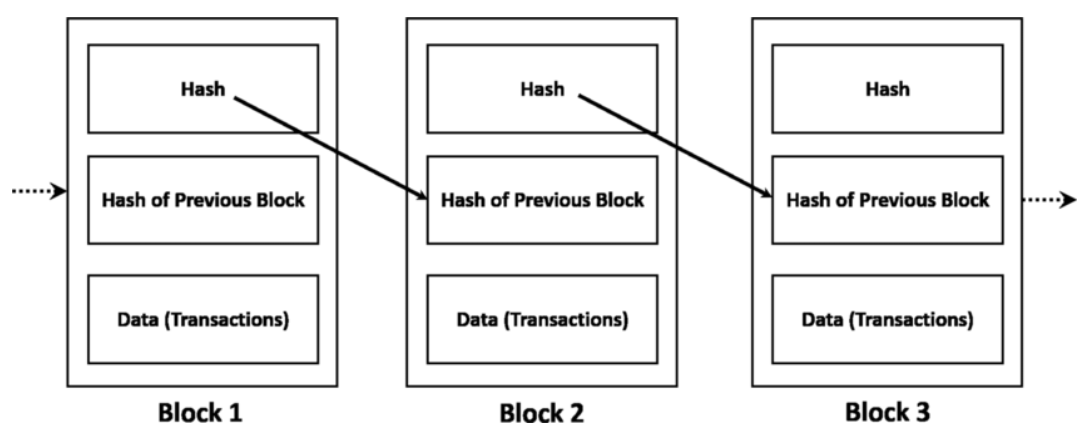
\includegraphics[width=0.8\textwidth]{../../img/Blockchain.png}
    \caption{Esempio di architettura di una blockchain}
    \label{fig:Blockchain}
\end{figure}
Le blockchain possono essere categorizzate in tre tipi principali \cite{Tassonomia}:
\begin{itemize}
    \item \textbf{Blockchain pubbliche}: sono blockchain che chiunque nel mondo può leggere, inviare transazioni e controllare se le transazioni sono valide. Tutti i nodi della rete possono partecipare al processo di consenso e alla validazione delle transazioni. Queste blockchain vengono considerate totalmente decentralizzate. Un esempio di blockchain pubblica è Bitcoin.
    \item \textbf{Blockchain private}: sono blockchain in cui l'accesso ai permessi di scrittura è tenuto centralizzato ad una organizzazione. I permessi di lettura potrebbero essere pubblici o ristretti ad un gruppo selezionato di utenti. Un esempio di applicazioni di questo tipo possono essere quelle utilizzate in ambito aziendale.
    \item \textbf{Blockchain consorziate}: sono blockchain in cui il processo di consenso è controllato da un numero limitato di nodi; ad esempio si può pensare ad un consorzio di istituzioni finanziare in cui ognuna opera come un nodo della rete e per raggiungere un consenso è necessario che la maggioranza dei nodi sia d'accordo. Queste blockchain vengono considerate parzialmente decentralizzate.
\end{itemize}
Una delle sfide principali della blockchain (ed in generale dei sistemi distribuiti) è il problema del consenso. Poichè nella blockchain non ci sonno dei nodi centrali che garantiscano che i ledger nei nodi distribuiti siano tutti uguali, è necessario che ci sia un protocollo che assicuri che i ledger siano consistenti tra i vari nodi. Questo protocollo è chiamato protocollo di consenso. Esistono diversi protocolli di consenso, tra i principali possiamo citare:
\begin{itemize}
    \item \textbf{Proof of Work (PoW)}: è il protocollo di consenso utilizzato da Bitcoin. Nel proof of work, i nodi della rete dimostrano che non siano dei malintenzionati spendendo una grande quantità di lavoro. Questo lavoro è fatto risolvendo un problema crittografico complesso. Nel PoW, ogni nodo della rete calcola l'hash del blocco, che deve però contenere un nonce ed essere più piccolo di un certo valore. Quando un nodo trova un hash che soddisfa questi requisiti,il blocco viene inviato a tutti gli altri nodi nella rete che devono confermare che il blocco sia valido. Questo processo è chiamato "mining" e i nodi che lo fanno sono chiamati "minatori". Quando un blocco viene confermato, il nodo che ha trovato il blocco riceve una ricompensa in criptovaluta.
    \item \textbf{Proof of Stake (PoS)}: è un protocollo di consenso alternativo a PoW. Poichè la PoW richiede una grande quantità di lavoro e di energia elettica, è stato proposto un protocollo di consenso alternativo che si basa sulla quantità di criptovaluta posseduta da un nodo. L'idea di base di PoS è che i nodi che possiedono una grande quantità di criptovaluta sono meno propensi a compiere azioni malevole, poichè ciò potrebbe danneggiare il valore della criptovaluta che possiedono. In PoS, i nodi sono selezionati per validare i blocchi in base alla quantità di criptovaluta che possiedono. Poichè basarsi solo sulla quantità di criptovaluta posseduta potrebbe portare a una centralizzazione del processo di consenso, sono stati proposti diversi algoritmi per selezionare i nodi in modo casuale. Ad esempio, Blackcoin \cite{Blackcoin} utilizza un algoritmo di selezione casuale basato su una lotteria; Peercoin \cite{Peercoin} utilizza un algoritmo di selezione casuale basato sulla quantità di criptovaluta posseduta oltre che sulla quantità di tempo a partire da cui la criptovaluta è stata posseduta. Al contrario di PoW, PoS non richiede una grande quantità di lavoro e di energia elettrica, rendendo il processo di consenso più efficiente e sostenibile, ma più il costo per il mining di un  scende, più aumentano le probabilità di attacchi alla blockchain. 
    \item \textbf{Delegated Proof of Stake (DPoS)}: è una variante di PoS in cui i possessori di criptovaluta possono votare per i nodi che desiderano che validino i blocchi. I nodi più votati vengono selezionati per validare i blocchi. Questo riduce il numero di nodi che devono essere coinvolti nel processo di consenso.
\end{itemize}
Questi protocolli sono solo alcuni dei tanti protocolli di consenso che sono stati proposti. Ogni protocollo ha i suoi vantaggi e svantaggi e può essere adatto a diversi contesti e applicazioni.
\subsection{Ethereum}
Tra le principali blockchain pubbliche, una delle più importanti è Ethereum. Ethereum è una piattaforma open-source basata su blockchain che permette di creare e distribuire applicazioni decentralizzate. Ethereum è stata proposta per la prima volta nel 2014 da Vitalik Buterin \cite{Ethereum}. Ethereum è simile a Bitcoin, ma ha alcune differenze chiave, si può dire che ethereum estende i concetti proposti da Bitcoin. Mentre Bitcoin è progettato principalmente per essere una valuta digitale, Ethereum è progettato per essere una piattaforma per la creazione di applicazioni decentralizzate. Ethereum ha una propria criptovaluta, chiamata Ether, che viene utilizzata per pagare le transazioni sulla rete. La blockchain di Ethereum è pubblica e permissionless, il che significa che chiunque può partecipare alla rete e inviare transazioni. Ethereum utilizza un protocollo di consenso chiamato Proof of Work, ma è in fase di transizione verso un protocollo di consenso chiamato Proof of Stake.

\subsection{Smart Contracts}

La principale innovazione di Ethereum è l'introduzione degli Smart Contracts.
Gli smart contracts sono programmi che vengono memorizzati ed eseguiti su una blockchain, possono essere definiti come dei contenitori di codice che incaplusano e replicano i termini di contratti del mondo reale in un dominio digitale \cite{SCReview}. Essi agiscono come accordi  che aiutano a scambiare denaro, proprietà, azioni o qualsiasi cosa di valore in modo trasparente, eliminando la necessità di un intermediario. Gli smart contracts sono eseguiti automaticamente quando vengono soddisfatte determinate condizioni. Ad esempio, un contratto di assicurazione potrebbe pagare automaticamente un risarcimento se si verifica un determinato evento. Poichè gli smart contracts sono accessibili ad entrambe le parti non ci sono dispute una volta che il contratto è stabilito. 

Gli Smart Contracts Ethereum possono essere visti come degli agenti autonomi che vivono sulla blockchain Ethereum. Essi possono inviare e ricevere transazioni, memorizzare dati e interagire con altri contratti. Gli Smart Contracts sono scritti in un linguaggio di programmazione chiamato Solidity, che è stato progettato appositamente per la creazione di Smart Contracts. Solidity è un linguaggio di programmazione Turing-completo ad alto livello, progettato per essere eseguito sulla blockchain Ethereum. Gli Smart Contracts Ethereum sono eseguiti su una macchina virtuale chiamata Ethereum Virtual Machine (EVM). L'EVM è una macchina virtuale Turing-completa che esegue il codice Solidity e garantisce che il codice sia eseguito in modo deterministico e sicuro. 

Poichè gli Smart Contracts vengono eseguiti sulla blockchain e sono Turing-completi sono soggetti all'Halting problem, cioè non è possibile sapere a priori se un'esecuzione di un contratto terminerà o meno. Questo renderebbe le Blockchain facilmente soggette a attacchi di tipo Denial of Service. Per evitare questo problema, Ethereum ha introdotto il concetto di gas. Il gas è una misura dell'uso delle risorse computazionali e di memoria di un contratto. Ogni operazione che un contratto esegue costa una certa quantità di gas. Gli utenti che inviano transazioni devono specificare il prezzo del gas che sono disposti a pagare per l'esecuzione della transazione. Se il gas fornito non è sufficiente per completare l'esecuzione del contratto, la transazione viene annullata e il gas speso non viene restituito all'utente. Al contrario, se l'utente consuma meno del massimo gas disponibile l'eccedenza viene restituita al proprietario. Questo meccanismo garantisce che i contratti non possano eseguire operazioni infinite e che gli utenti non possano abusare della rete Ethereum inviando transazioni che richiedono una grande quantità di risorse computazionali.

\subsection{Vulnerabilità negli Smart Contracts}
Poichè gli Smart Contracts sono eseguiti su una blockchain pubblica e sono accessibili a tutti, è importante garantire che siano sicuri e privi di vulnerabilità. Una delle caratteristiche principali delli smart contracts è la loro immutabilità. Una volta che un contratto è stato pubblicato sulla blockchain, non può essere modificato o cancellato. Questa proprietà assicura che il comportamento del contratto sia prevedibile e che le parti coinvolte possano fidarsi del contratto. Tuttavia, questa proprietà rende anche gli Smart Contracts vulnerabili a errori e vulnerabilità. Se un contratto contiene una vulnerabilità, non può essere corretto e rimarrà vulnerabile per sempre. Questo rende gli Smart Contracts un obiettivo attraente per gli attaccanti che possono sfruttare le vulnerabilità negli Smart Contracts per rubare fondi, bloccare i fondi o causare altri danni. Le vulnerabilità negli Smart Contracts possono essere di diversi tipi, tra cui vulnerabilità di accesso, vulnerabilità di overflow/underflow, vulnerabilità di reentrancy e vulnerabilità di arithmetic. Queste vulnerabilità possono portare a perdite finanziarie, a blocchi della blockchain e ad altri problemi. Per questo motivo, è importante che gli Smart Contracts siano sicuri e privi di vulnerabilità.

Di seguito presenteremo alcune tra le principali classi di vulnerabilità a cui gli smart contracts sono esposti.

\subsubsection{Access-Control}
La vulnerabilità di access control è una vulnerabilità presente non solo in Solidity ma in numerosi altri linguaggi di programmazione. Questa vulnerabilità si verifica quando un contratto non controlla correttamente l'accesso alle sue funzioni e ai suoi dati, è quindi una vulnerabilità legata al governanre chi può interagire con le varie funzionalità all'interno del contratto. Un esempio di questo dipo di vulnerabilità è legato alla mancata restrizione dell'accesso a funzioni di inizializzazione, ad esempio:
\begin{lstlisting}[language=Solidity]
function initContract() public {
    owner = msg.sender;
}
\end{lstlisting} 
Questa funzione serve a inizializzare l'owner del contratto, ma non controlla chi può chiamarla, permettendo a chiunque di chiamarla e diventare l'owner del contratto e non ha nemmeno controlli per prevenire la reinizializzazione. Questo è un esempio molto semplice di come una vulnerabilità di access control possa portare a comportamenti inaspettati. 
Un famoso attacco che ha subito una vulnerabilità di tipo access-control è il caso di Parity Multisig Wallet, un contratto che permetteva di creare wallet multi firma. Questo contratto ha subito un attacco nel Luglio 2017 che ha portato alla perdita di una grande quantità di Ether. L'attacco è stato effettuato da un utente che ha sfruttato una vulnerabilità di access control per diventare l'owner del contratto e rubare criptovalute ad altri utenti, si stima che la perdita sia stata di circa 30 milioni di dollari.


\subsubsection{Arithmetic}
Le vulnerabilità di tipo aritmetico \cite{sc-vulnerabilities} sono vulnerabilità che vengono generate come risultato di operazioni matematiche. Una delle vulnerabilità più significative all'interno di questa classe è rappresentata dagli underflow/overflow, un problema molto comune nei linguaggi di programmazione. Incrementi di valore di una variabile oltre il valore massimo rappresentabile o decrementi al di sotto del valore minimo rappresentabile (detti \emph{wrap around}) possono generare comportamenti indesiderati e risultati errati. In tutte le versioni di Solidity precedenti alla versione 0.8.0, le operazioni aritmetiche non controllano i limiti di overflow e underflow previsti per quel tipo di dato (es.uint64 o uint256), permettendo a un attaccante di sfruttare questa vulnerabilità per ottenere un vantaggio. Ad esempio nel caso in cui si stia utilizzano un uint256 il massimo numero che si piuò memorizzare nella variabile è $2^256 - 1$, che è un numero molto alto, ma resta comunque possibile superare questo limite, facendo entrare in scena l'overflow. Quando si verifica un overflow, il valore della variabile riparte dal piuù piccolo valore rappresentabile. Questo può portare a comportamenti inaspettati e a perdite di fondi. Vediamo un esempio molto banale di contratto vulnerabile:
\begin{lstlisting}[language=Solidity]
    pragma solidity 0.7.0;

    contract ChangeBalance {
        uint8 public balance;
        function decrease() public {
            balance--;
        }
        function increase() public {
            balance++;
        }
    }
\end{lstlisting}
Questo codice rappresenta un contratto che molto semplicemente memorizza un saldo all'interno di una variabile di tipo uint8, cioè un intero a 8bit ovvero un intero che può memorizzare valori da 0 a $2^8-1$, quindi da 0 a 255. Se un utente chiamasse la funzione \texttt{increase()} in modo tale che faccia salire il valore del saldo a $256$ il calcolo risulterebbe in un overflow e il valore della variabile ritornerebbe a 0. Questo è un esempio molto semplice di come un overflow possa portare a comportamenti inaspettati. L'underflow si verificherebbe nel caso diametralmenmte opposto, in cui viene chiamata la funzione \texttt{decrease()} quando il saldo è a 0. In questo caso il valore della variabile ritornerebbe a 255.
Un esempio di attacco che sfrutta l'overflow è stato l'attacco del 23 Aprile 2018 effettuato su uno smart contract di BeautyChain (BEC) che ha causato un importantissimo crash del prezzo. La funzione che ha causato l'overflow permetteva di trasferire una certa somma di denaro presa in input a più utenti contemporaneamnete e per farlo controllava dapprima che il saldo del contratto fosse maggiore o uguale alla somma da trasferire:
\begin{lstlisting}[language=Solidity]
    function batchTransfer(address[] _receivers, uint256 _value) public whenNotPaused returns (bool) {
        uint cnt = _receivers.length;
        uint256 amount = uint256(cnt) * _value;
        require(cnt > 0 && cnt <= 20);
        require(_value > 0 && balances[msg.sender] >= amount);
    
        balances[msg.sender] = balances[msg.sender].sub(amount);
        for (uint i = 0; i < cnt; i++) {
            balances[_receivers[i]] = balances[_receivers[i]].add(_value);
            Transfer(msg.sender, _receivers[i], _value);
        }
        return true;
     }
\end{lstlisting}
% IMAGE BECPrice
\begin{figure}[H]
    \centering
    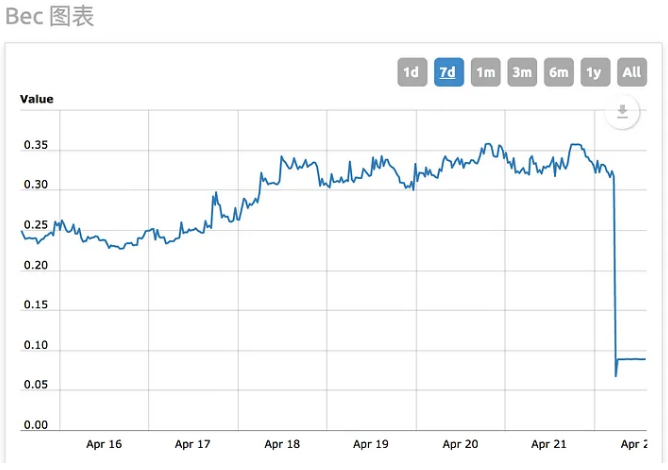
\includegraphics[width=0.8\textwidth]{../../img/BECPrice.png}
    \caption{Andamento del prezzo di BEC prima e dopo  l'attacco}
    \label{fig:BECPrice}
\end{figure}
Dalla versione di Solidity 8.0  tutti i calcoli che superano i limiti di rappresentazione del tipo di dato vengono interrotti e viene lanciata un'eccezione. Questo permette di evitare che si verifichino overflow e underflow. Un'altra soluzione a questo tipo di errori è l'utilizzo della libreria SafeMath, che offre operazioni aritmetiche che controllano i limiti di rappresentazione del tipo di dato prima di effettuare i calcoli. Overflow e underflow sono le principali vulnerabilità di tipo aritmetico, ma non sono le uniche. Un'altra vulnerabilità di tipo aritmetico è rappresentata dalla divisione per zero. In Solidity nelle versioni precedenti alla 0.4 la divisione per zero non lancia un'eccezione, ma ritorna il valore 0, questo può portare a comportamenti inaspettati e a perdite di fondi.
\subsubsection{Other}
In questa classe di vulnerabilità rientrano tutte quelle vulnerabilità che non fanno parte delle altre classi. Uno degli esempi sono le vulnerabilità di \emph{uninitialized-state} che fanno capo a tutte quelle vulnerabilità a seguito di variabili che non vengono inizializzate correttamente. Le variabili in Solidity possono essere memorizzate in \emph{memory}, \emph{storage} o \emph{calldata}. Bisogna assicurarsi che questi diversi storage vengano compresi e inizializzati correttamente, poichè ad esempio inzializzare male i puntatori allo storage o lasciarli non inizializzati può portare a degli errori. Da Solidity 0.5.0 i puntatori allo storage non inizializzati non sono più un problema poichè contratti con puntatori non inizializzati risulteranno in errori di compilazione.  
Un altra possibile vulnerabilità è detta \emph{incorrect-equality}. Questa vulnerabilità si verifica, solitamente, quando si controlla affinche un account ha abbastanza Ether o Tokens utilizzando una uguaglianza stretta, ciò è un qualcosa che un soggetto malevolo può facilmente manipolare per attaccare il contratto. Un esempio di questo tipo di vulnerabilità è il caso in cui il contratto entra in uno stato di \emph{GridLock}:
\begin{lstlisting}[language=Solidity]
    /**
    * @dev        Locks up the value sent to contract in a new Lock
    * @param      term         The length of the lock up
    * @param      edgewareAddr The bytes representation of the target edgeware key
    * @param      isValidator  Indicates if sender wishes to be a validator
    */
   function lock(Term term, bytes calldata edgewareAddr, bool isValidator)
       external
       payable
       didStart
       didNotEnd
   {
       uint256 eth = msg.value;
       address owner = msg.sender;
       uint256 unlockTime = unlockTimeForTerm(term);
       // Create ETH lock contract
       Lock lockAddr = (new Lock).value(eth)(owner, unlockTime);
       // ensure lock contract has all ETH, or fail
       assert(address(lockAddr).balance == msg.value); // BUG
       emit Locked(owner, eth, lockAddr, term, edgewareAddr, isValidator, now);
   }
\end{lstlisting}
In questo caso la vulnerabilità è rappresentata dall'assert che controlla che il contratto abbia ricevuto la quantità di Ether corretta. Il controllo si basa sull'assunzione che il contratto essendo creato alla riga precedente abbia saldo zero ed essendo precaricato proprio con \emph{msg.value} si suppone che il saldo del contratto sia uguale a \emph{msg.value}. In realtà gli Ether possono essere inviati ai contratti prima che vengano istanziati negli indirizzi stessi, poichè la generazione degli indirizzi dei contratti in Ethereum è un processo basato su dei nonce deterministici. L'attacco DoS che si basa su questa vulnerabilità in questo caso consiste nel pre-calcolare l'indirizzo del contatto \emph{Lock} e mandare dei Wei a quell'indirizzo. Questo forza la funzione \emph{lock} a fallire e a non creare il contratto, bloccando il contratto in uno stato di \emph{GridLock}.  Per risolvere questa problematica, si potrebbe adottare l'approccio di sostituire l'uguaglianza stretta con un confronto maggiore o uguale. 
\subsubsection{Reentrancy}
La Reentrancy è una classe di vulnerabilità presente negli SmartContracts che permette ad un malintenzionato di rientrare nel contratto in modo inaspettato durante l'esecuzione della funzione originale. Questa vulnerabilità può essere utilizzata per rubare fondi e rappresenta la vulnerabilità più impattante dal punto di vista di perdita di fondi a seguito di attacchi.
Il caso più famoso di questo attacco che lo ha anche reso noto è il caso di The DAO, un contratto che ha subito un attacco di reentrancy che ha portato alla perdita circa sessanta milioni di dollari in Ether, circa il 14\% di tutti gli Ether in circolazione all'epoca. Nonostante dal 2016 ad oggi siano stati fatti numerosi progressi nelle tecnologie e nelle misure di sicurezza questa vulnerabilità rimane comunque una delle minacce più pericolose per gli SmartContracts, poichè negli anni questo tipo di attacchi si è ripresentato notevole frequenza \cite{reentrancy-historical}. Un attacco di reentrancy può essere classificato in tre classi differenti:
\begin{itemize}
    \item \textbf{Mono-Function}: la funzione vulnerabile è la stesa che viene chiamata più volte dall'attaccante, prima del completamento delle sue invocazioni precedenti. Questo è il caso più semplice di attacco reentrancy e di conseguenza il più facile da individuare.
    \item \textbf{Cross-Function}: questo caso è molto simile al caso di mono-function Reentrancy, ma in questo caso la funzione che viene chiamata dall'attaccante non è la stessa che fa la chiamata esterna. Questo tipo di attacco è possibile solo quando una funzione vulnerabile condivide il suo stato con un'altra funzione, risultando in un una situazione fortemente vantaggiosa per l'attaccante. 
    \item \textbf{Cross-Contract}: questo tipo di attacco prende piede quando lo stato di un contratto è invocato in un altro contratto prima che viene correttamente aggiornato. Avviene solitamente quando più contratti condividono una variabile di stato comune e uno di loro la aggiorna in modo non sicuro. 
\end{itemize}
Mostreremo adesso alcuni esempi di contratti vulnerabili a questo tipo di attacco. 
\begin{lstlisting}[language=Solidity]
// UNSECURE
function withdraw() external {
    uint256 amount = balances[msg.sender];
    (bool success,) = msg.sender.call{value: balances[msg.sender]}("");
    require(success);
    balances[msg.sender] = 0;
}
\end{lstlisting}
In questo caso, il balance dell'utente viene aggiornato solo dopo che la chiamata esterna è stata completata. Questo permette all'attaccante di chiamare la funzione withdraw più volte prima che il balance venga settato a zero, permettendo all'attaccante di rubare fondi allo smart contract.
Una versione più complessa dello stesso processo è il caso cross function, di cui mostriamo un esempio:
\begin{lstlisting}[language=Solidity]
    // UNSECURE
function transfer(address to, uint amount) external {
  if (balances[msg.sender] >= amount) {
    balances[to] += amount;
    balances[msg.sender] -= amount;
  }
}

function withdraw() external {
  uint256 amount = balances[msg.sender];
  (bool success,) = msg.sender.call{value: balances[msg.sender]}("");
  require(success);
  balances[msg.sender] = 0;
}
\end{lstlisting}
In questo esempio, l'attaccante può effettuare un attacco di tipo reentrancy avendo una avendo una funzione che chiama \texttt{transfer()} per trasferire fondi spesi prima che il bilancio sia settato a zero dalla funzione \texttt{withdraw()}.
Un nuovo tipo di attacchi sono gli attacchi Read-only Reentrancy, in 
\subsubsection{Unchecked-Calls}
In solidity si possono usare delle chiamate a funzione low level come `address.call()`




\section{Lavori Correlati}
\label{ch:relatedwork}
Il tema della rilevazione delle vulnerabilità all'interno degli Smart Contracts è un tema che ha guadagnato notevole importanza nel tempo, anche a seguito della grande diffusione della tecnologia blockhain. Proprio per questo motivo, sono stati sviluppati e proposti diversi approcci per la rilevazione automatica di vulnerabilità all'interno degli Smart Contracts. In questo capitolo verranno presentati alcuni dei lavori più significativi che si sono occupati di questo tema.
Tra i principali approcci proposti figurano gli approcci basati su analisi statica basati su tecniche di esecuzione simbolica. L'analisi statica si basa sull'esame del codice sorgente o bytecode di uno smart contract senza effettuarne l'esecuzione effettiva. Questo approccio consente di identificare potenziali problematiche senza la necessità di testare il codice in un ambiente reale. L'esecuzione simbolica è una tecnica particolarmente potente in questo contesto in quanto consente di esplorare tutte le possibili esecuzioni del programma, consentendo di individuare vulnerabilità che potrebbero emergere solo in determinate condizioni.
Gli approcci basati su esecuzione simbolica cercano di risolvere queste vulnerabilità attraverso la generazione di un grafo di esecuzione simbolico, in cui le variabili sono rappresentate come simboli e le esecuzioni possibili del programma vengono esplorate simbolicamente. Ciò consente di identificare percorsi di esecuzione che potrebbero condurre a condizioni di errore o vulnerabilità.
Tuttavia, va notato che l'analisi statica, inclusa l'esecuzione simbolica, può essere complessa e non sempre completa. Alcune vulnerabilità potrebbero sfuggire a questa analisi o richiedere ulteriori tecniche di verifica. Pertanto, è consigliabile combinare l'analisi statica con altre metodologie, come l'analisi dinamica e i test formali, per garantire una copertura completa nella rilevazione di vulnerabilità negli smart contract. Tra i principali strumenti che utilizzano questo tipo di analisi ci sono Maian \cite{Maian, Maian2}, Oyente \cite{Oyente, Oyente2}, Mythril \cite{Mythril}, Manticore \cite{Manticore} e altri.
Un'altro tipo di approcci ad analisi statica sono i tools basati su regole. Questi strumenti usano un set di regole predefinite e pattern per identificare delle potenziali nvulnerabilità nel codice sorgente. Questi tool analizzano il codice sorgente e segnalano tutte le istanze dove il codice viola delle regole predefinite. Le regole sono tipicamente basate su delle vulnerabilità note e delle best practice di programmazione, come ad esempio evitare dei buffer overflow, usare algoritmi di cifratura sicuri e validare propriamente l'input degli utenti. La limitazione principale di questi strumenti è che i risultati che producono sono limitati al set di regole che è stato implementato, quindi non riescono a riconoscere delle nuove vulnerabilità o vulnerabilità non scoperte precedentemente. Inoltre, un'altra grande limitazione di questi strumenti è il fatto che possano produrre un alto numero di falsi positivi, cioè di situazioni in cui il codice viene segnalato come codice vulnerabile ma in realtà è codice perfettamente sano. Tra i principali strumenti che utilizzano questo tipo di analisi ci sono Slither \cite{Slither}, Securify \cite{Securify}, SmartCheck \cite{SmartCheck} e altri.
Un'altra categoria di strumenti per la rilevazione di vulnerabilità negli smart contract sono gli approcci basati su tecniche di Machine Learning e Deep Learning, tra le quali anche il lavoro di questa tesi va ad inserirsi. Un approccio basato sulla trasformazione degli opcode dei contratti e la sua relativa analisi con dei modelli di Machine Learning tradizionale è stato offerto da Wang et al. \cite{ContractWard} i quali hanno raggiunto risultati eccellenti, con risultati in termini di F1 Score superiori al 95\% in quasi tutte le classi prese in analisi con il modello XGBoost che è risultato il miglior modello. Un altro lavoro che sfrutta tecniche di Machine Learning più tradizionali è il lavoro di Mezina e Ometov che hanno utilizzato classificatori come RandomForest, LogisticRegressio, KNN, SVM in un approccio dapprima binario (valutare se il contratto abbia o meno delle vulnerabilità) e poi multiclasse (valutare quale tipo di vulnerabilità il contratto abbia) \cite{Mezina}. I risultati in questo caso hanno mostrato come il modello SVM sia quello che ottiene i migliori risultati in termini di accuratezza. 

Spostandoci su lavori che utilizzano tecniche di Deep Learning è importante citare un'altro lavoro effettuato sullo stesso dataset su cui è basato questo lavoro di tesi. Questo dataset è stato infatti raccolto e pubblicato da un gruppo di ricercatori dell'Università di Bologna che ha effettuato un primo studio utilizzando un approccio basato su reti neurali convoluzionali \cite{RossiniPaper1}. L'approccio in questo caso è stato quello di classificare le vulnerabilità in un'impostazione multilabel del problema (in cui la label da predire è un array di elementi, quindi in cui il contratto può appartenere contemporaneamente a più classi) itilizzando delle reti neurali convoluzionali per la rilevazione delle vulnerabilità trasformando in codice Bytecode espresso in esadecimale dei contratti in delle immagini RGB. Questo lavoro ha  come risultato principale la dimostrazione che utilizzando delle reti neurali convoluzionali è possibile rilevare le vulnerabilità presenti negli SmartContracts con delle buone performance, i migliori risultati si attestano con un MicroF1 score del 0.83\% e mostrano come i migliori risultati siano dati da delle resi Resnet con delle convoluzioni unidimensionali. Successivamente, gli stessi autori hanno pubblicato una seconda analisi effettuata sul dataset utilizzando nuovi classificatori come CodeNet, SvinV2-T e Inception, mostrando come i migliori risultati  continuino ad essere quelli forniti da reti convoluzionali unidimensionali \cite{RossiniPaper2}. Altri lavori che utilizzano un approccio basato su tecniche di Deep Learning è il lavoro proposto da Huang \cite{Huang} che utilizza anch'egli delle reti neurali convoluzionali per la rilevazione delle vulnerabilità. I modelli utilizzati sono modelli molto noti come Alexnet, GoogleNet e Inception v3, i risultati migliori in questo caso si attestano sul 75\%.
Un importante lavoro offerto da Deng et Al. \cite{Deng} ha proposto un approccio basato sulla fusione di feature multimodali, analizzando contemporaneamente codice sorgente, bytecod e grafi di controllo del flusso. Per ognuna di queste tre feature è stato trainato un semplice classificatore con una rete neurale feedforward e sono poi state combinate le predizioni di questi tre classificatori in un classificatore finale utilizzando un approccio di ensamble learning detto stacking. I risultati ottenuti mostrano come l'approccio proposto abbia ottenuto dei risultati migliori rispetto ad un approccio in cui si utilizzava solo una delle tre feature.


\end{document}